\documentclass[mathserif,serif,handout]{beamer}

\setbeamertemplate{navigation symbols}{}

\usepackage{xcolor}

\definecolor{purple}{RGB}{57,39,91}
\definecolor{lightpurple}{RGB}{223,221,232}
\definecolor{LightGray}{rgb}{0.90,0.90,0.90}

\setbeamercolor{title}{fg=purple}
\setbeamercolor{titlelike}{fg=purple}
\setbeamercolor{background canvas}{bg=white}
\setbeamercolor{item projected}{fg=purple}
\setbeamercolor{item}{fg=purple}
\setbeamercolor{caption name}{fg=purple}

% Explainframes:
\usepackage{ifthen}
\newboolean{isexplainframe}
\setboolean{isexplainframe}{false}
\mode<handout>{
\newenvironment{explainframe}[1]{
\setboolean{isexplainframe}{true}
\addtocounter{framenumber}{-1}
\setbeamertemplate{background}[grid][step=5mm,color=LightGray]
\begin{frame}{Handout only: #1}%
}{%
\end{frame}%
\setboolean{isexplainframe}{false}
}}
\mode<beamer>{
\excludecomment{explainframe}
}

\title[Query Visualization] % (optional, only for long titles)
{Visualizing Physical Query Execution in a Relational Distributed Big Data Management System}
\subtitle{}
\author[Chu, moritz] % (optional, for multiple authors)
{Shumo Chu, Dominik Moritz}

\begin{document}

\begin{frame}
\titlepage

\end{frame}

\begin{frame}
\frametitle{Objective}
\begin{enumerate}
	\item 
\end{enumerate}
\end{frame}

\begin{frame}
\frametitle{The Myria System}
\begin{enumerate}
	\item Big Data management system developed in db group
	\item Pipelined, parallel, distributed dataflow evaluation system
	\item \textbf{Fragments}: trees of operators that are each executed on one thread in each worker
	\item Fragment leaves and roots are typically I/O operators
\end{enumerate}
\end{frame}

\begin{frame}
\frametitle{Myria Architecture}
\begin{figure}
 \begin{center}
     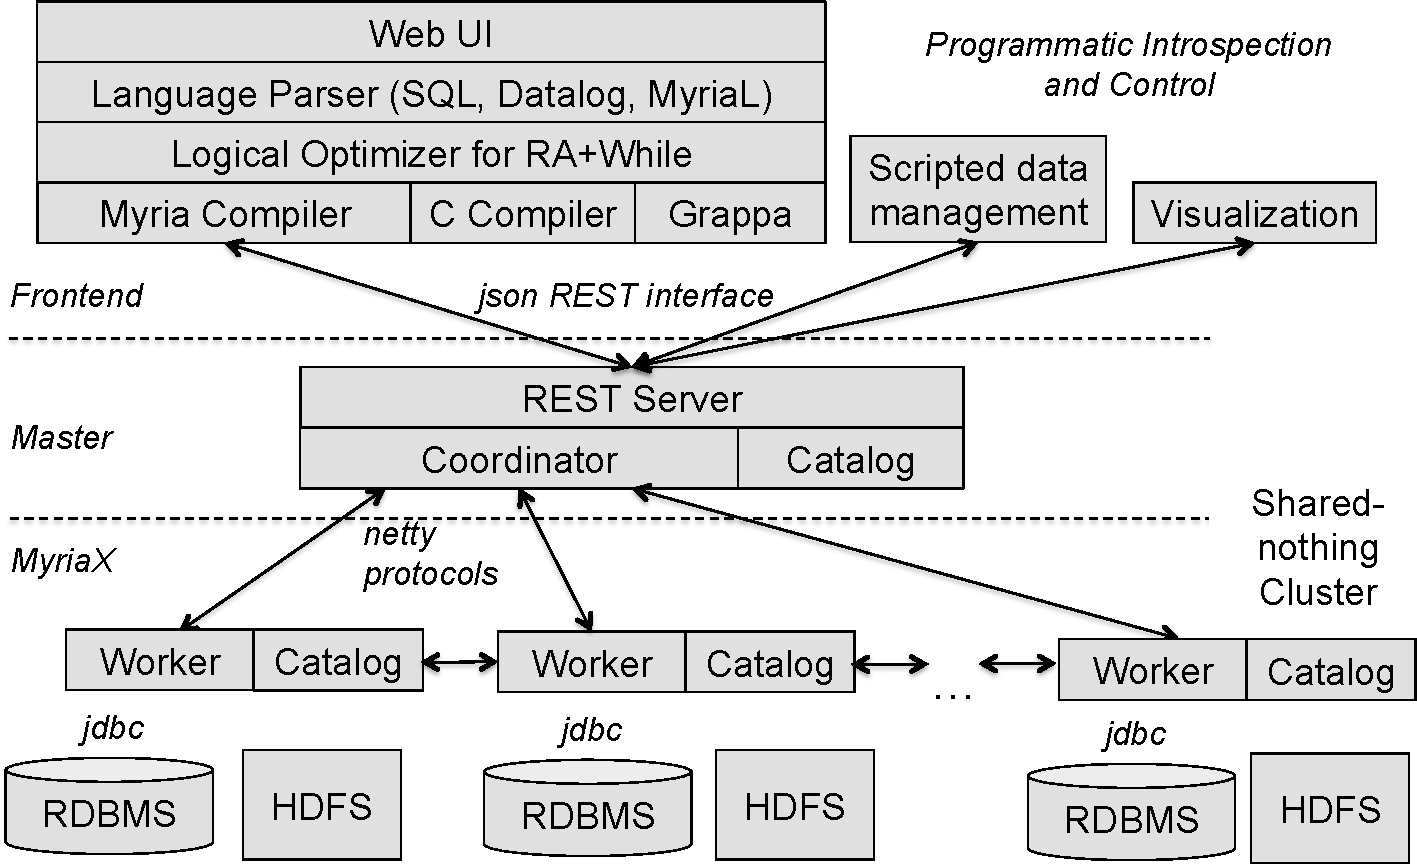
\includegraphics[width=0.9\textwidth]{arch}
   \end{center}
  \caption{Myria System Architecture.}
  \label{fig:myria_arc}
\end{figure}
\end{frame}

\begin{frame}
\frametitle{System overview}
Image that shows how we fetch logs and where app engine is.
\end{frame}

\begin{frame}
\frametitle{Visualization: System Architecture}
\begin{figure}
	 \begin{center}
     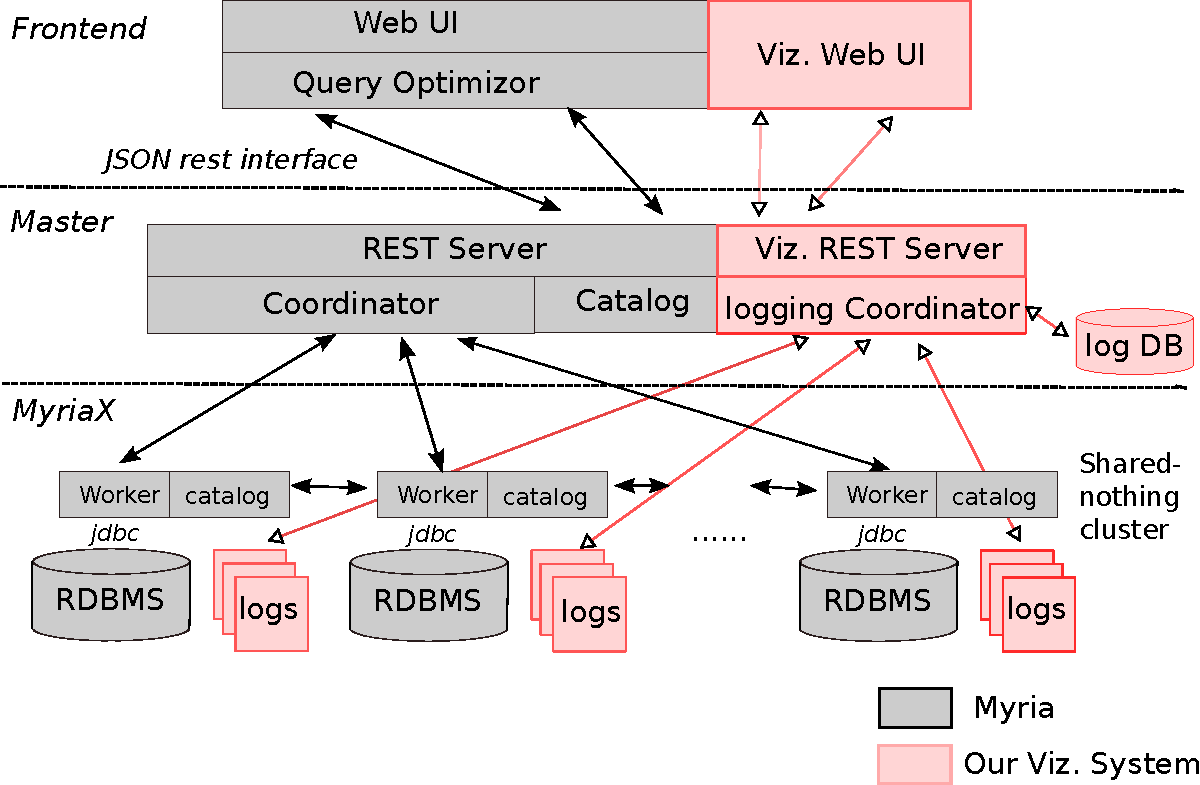
\includegraphics[width=0.9\textwidth]{viz_arch.pdf}
   \end{center}
   \caption{Visualization System Architecture.}
  \label{fig:viz_arc}
\end{figure}
\end{frame}

\begin{explainframe}{Query plan level visualization}
\end{explainframe}

\begin{explainframe}{Query fragment level visualization}
\end{explainframe}

\begin{explainframe}{Operator level visualization}
\end{explainframe}

\begin{frame}
\frametitle{Demo}
\begin{figure}
 \begin{center}
     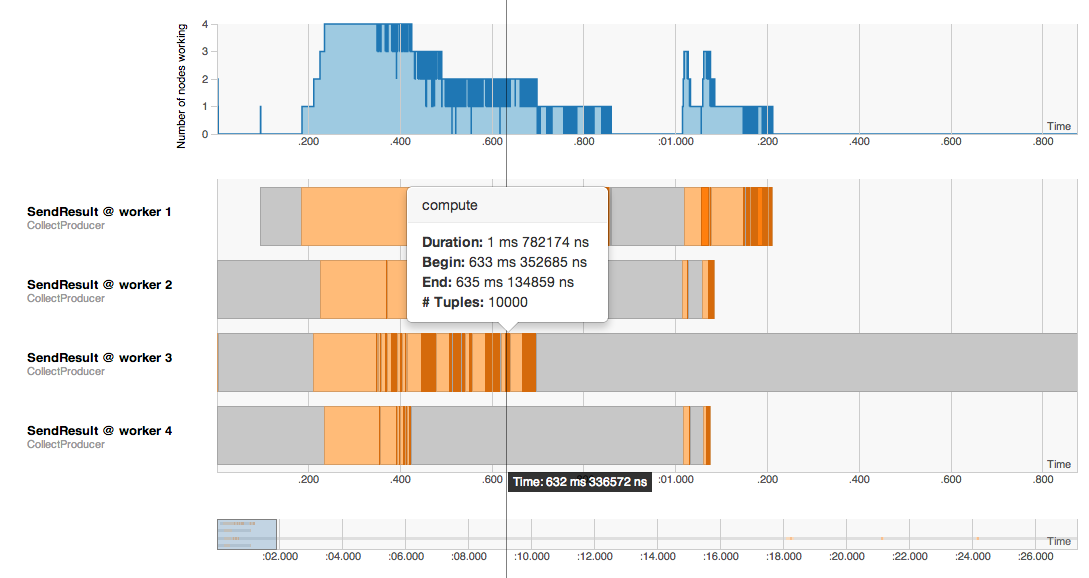
\includegraphics[width=\textwidth]{figure1}
   \end{center}
  \caption{Query fragment level visualization.}
\end{figure}
\end{frame}

\end{document}